En ésta sección se explicará en detalle el diseño estructural del sistema.  Cada una de las partes a detallar se dividirá a su vez en varias partes:
\begin{itemize}
	\item Se incluirá un diagrama que muestre de forma gráfica el diseño del componente y sus subcomponentes
	\item Se dará una explicación textual de los diferentes subcomponentes y las tareas que realizan
	\item Se dará una explicación textual sobre cómo se relacionan los subcomponentes entre sí
	\item Se describirá de forma detallada las interfaces y puertos utilizadas por los subcomponentes.  Las interfaces y puertos se dividirán en tablas por componentes para hacer más sencilla su lectura.	Cada entrada constará de los siguientes apartados:
	\begin{itemize}
		\item \textbf{Interfaz}.  Será el nombre que recibe el puerto/interfaz en el diagrama de componentes.
		\item \textbf{Tipo}.  El tipo de la interfaz/puerto será \textit{proveído} cuando se exponga una interfaz para su uso por parte de otro componente, o \textit{requerido} cuando se utilice una interfaz expuesta por otro componente.
		\item \textbf{Tecnología}.  Indica el tipo de tecnología de la interfaz/puerto.
		\item \textbf{Propiedades}.  Explica brevemente el objetivo de la interfaz/puerto.
	\end{itemize}
\end{itemize}

Es importante destacar que ésta sección se centrará en el subsistema de datos puesto que, como ya se ha mencionado en la sección \nameref{identificacion_subsistemas} perteneciente al capítulo \ref{chapter04}, los subsistemas pertenecientes a la zona social (subsistema de gestión de usuarios, eventos, noticias, debates, entradas del blog y comentarios) delegan su funcionalidad en componentes ya implementados por el gestor de contenidos.  De la misma forma, el subsistema de búsqueda delega su funcionalidad principal en el servidor de búsqueda.

\subsection{Vista del sistema}
\label{vista_sistema}
A continuación se detallará la estructura completa del sistema que forma el nuevo \textit{Land Portal}.  A pesar de que varios de los componentes que se verán aquí quedan fuera del ámbito de este proyecto, se ha decidido incluir esta vista para proveer de un contexto que permita al lector comprender en qué parte del sistema se situarán las vistas posteriores.

\subsubsection{Diagrama de componentes}
La figura \ref{fig:diagrama_componentes_sistema} muestra el diagrama de todos los componentes que conforman el nuevo \textit{Land Portal}.
\begin{landscape}
	\begin{figure}[ht]
		\centering
		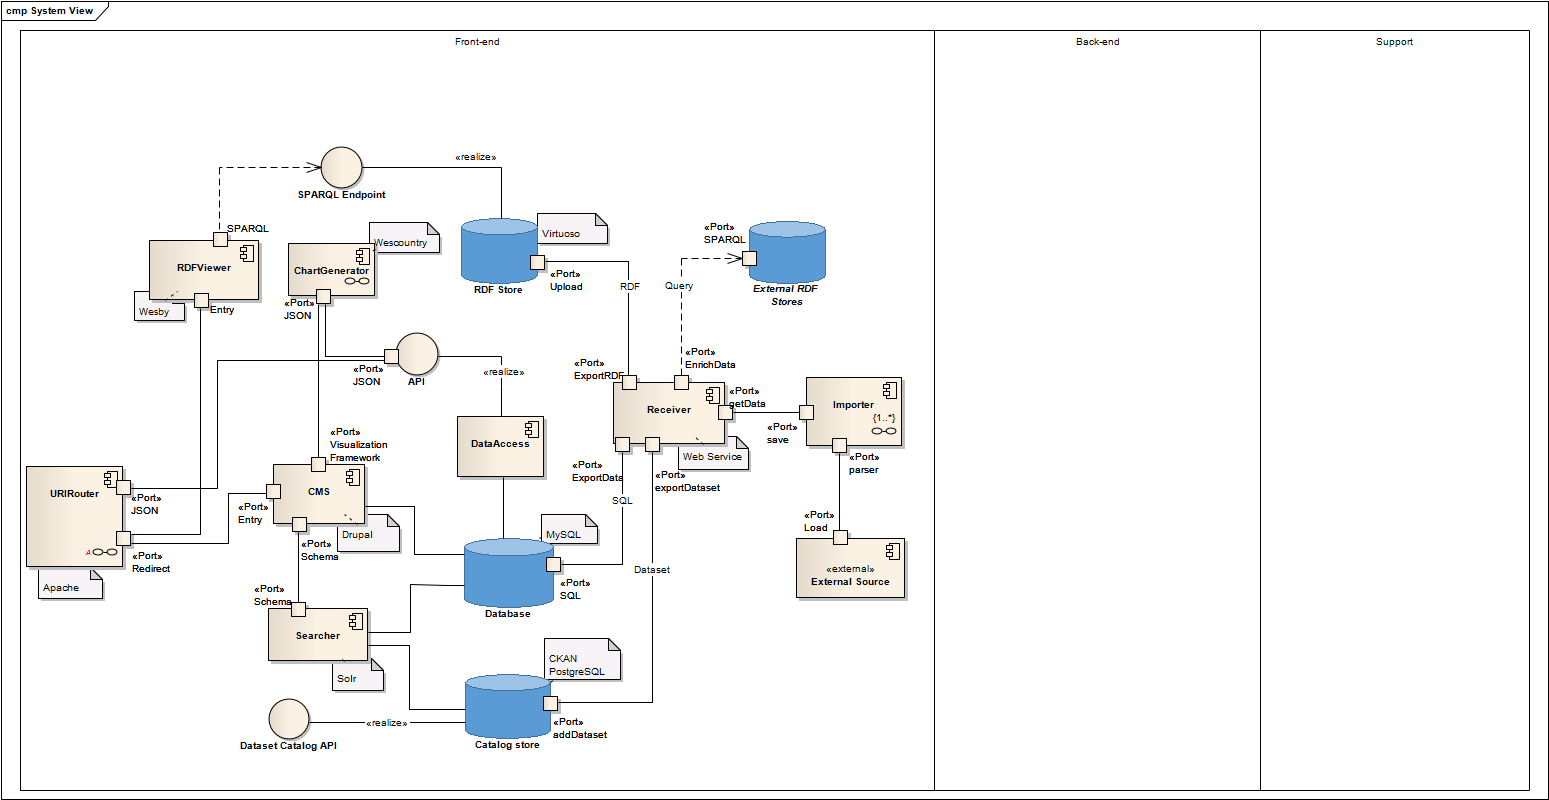
\includegraphics[height=\textwidth]{arquitectura/system_view}
		\caption{Diagrama de componentes del sistema}
		\label{fig:diagrama_componentes_sistema}
	\end{figure}
\end{landscape}


\subsubsection{Componentes}
Una vez mostrado el diagrama de componentes, se procederá a explicar el rol de cada uno de los componentes del sistema.  La descripción comenzará en los componentes más internos y terminará en los componentes más externos y cercanos al usuario del sistema.
\begin{description}
	\item[External source]  Las fuentes externas  serán fuentes de datos pertenecientes a organizaciones externas.  Estas fuentes proporcionan conjuntos de datos compuestos por indicadores y observaciones relativos a diferentes países y momentos del tiempo.  Como ya se ha mencionado en la sección ``\nameref{objetivos_proyecto}'' perteneciente al capítulo \ref{chapter01}, algunas de las fuentes externas con las que se trabajará son:
	\begin{itemize}
		\item el Banco Mundial (\textit{WorldBank})
		\item la Organización de las Naciones Unidas para la Alimentación y la Agricultura (\textit{FAO})
		\item la Organización Mundial de la Salud (\textit{WHO})
		\item el Instituto Internacional de Investigación sobre Políticas Alimentarias (\textit{IFPRI})
		\item la Organización para la Cooperación y el Desarrollo Económicos(\textit{OECD})
	\end{itemize}
	\item[Importer]  Los importadores  tendrán la tarea de transformar los conjuntos de datos provenientes de las fuentes externas a un formato común con el fin de unificar y asegurar un nivel de calidad mínimo para los datos que se insertarán en el portal.  Como se ha explicado en la sección ``\nameref{identificacion_actores}'' del capítulo \ref{chapter04}, los importadores serán los actores que interactuarán con el punto de entrada de datos, enviándole a este los conjuntos de datos ya procesados.
	\item[Receiver]  El Punto de Entrada de Datos  tendrá la misión de controlar todas las entradas de datos que se realicen hacia el portal.  Recibirá las peticiones de los importadores y almacenará los conjuntos de datos en varios servicios diferentes, concretamente: una base de datos SQL, una base de datos RDF y un catálogo de datos.  Además, el punto de entrada de datos también se encargará de enriquecer los datos antes de almacenarlos en el sistema, este enriquecimiento de datos tendrá lugar mediante la consulta de almacenamientos de RDF externos.  La arquitectura del punto de entrada de datos se verá con más detalle posteriormente en la sección ``\nameref{vista_receiver}'' de este mismo capítulo.
	\item[External RDF Stores]  Los almacenamientos (o \textit{endpoints}) de RDF externos son servicios externos que contienen información variada que se utilizará para enriquecer los datos que llegan al punto de entrada.  Un ejemplo de almacenamiento de RDF externo es \textit{DBPedia}\footnote{DBPedia contiene la información de la Wikipedia en forma de datos enlazados \url{http://dbpedia.org/About}}.
	\item[Database]  La base de datos será utilizada tanto por el gestor de contenidos y el framework de visualizaciones como por el API.  La base de datos será también uno de los lugares donde el punto de entrada almacene los catálogos de datos que llegan al portal.  El funcionamiento y esquema de la base de datos se detallará en la sección ``\nameref{diseno_modelo_datos}'' perteneciente a este mismo capítulo.
	\item[Catalog store - Dataset Catalog API]  El catálogo de datos será el encargado de almacenar los catálogos de datos que se utilizan en el portal acompañados de una serie de metadatos sobre su origen, creador, formato, etc.  Proveerá también una interfaz que permitirá a los usuarios navegar e incluso descargar en bruto los catálogos de datos almacenados en el sistema.  Como ya se explicó en la sección ``\nameref{chapter02:alternativas_seleccionadas}'' del capítulo \ref{chapter02}, el catálogo de datos seleccionado ha sido CKAN.  Al igual que la base de datos, el catálogo de datos será uno de los lugares en los que el punto de entrada almacena la información que llega al portal.
	\item[RDF Store - SPARQL endpoint]  El servidor semántico almacenará los datos en formato RDF y proveerá una punto de acceso SPARQL\footnote{SPARQL es un lenguaje de consultas capaz de manipular datos en formato RDF.  Para una mayor información al respecto véase \url{http://www.w3.org/TR/sparql11-overview/}} que podrá ser utilizado por los usuarios o por otros componentes del sistema.  Este componente será uno de los lugares donde el punto de entrada almacene los catálogos de datos que recibe.
	\item[API - DataAccess]  El API será el encargado de proporcionar una interfaz de acceso a los datos almacenados en la base de datos del sistema.  El API seguirá una arquitectura REST e incluirá un sistema de negociación de contenido con el que el cliente podrá seleccionar el formato en el que recibe los datos.  Algunos de los formatos soportados por el API serán JSON, CSV y XML.
	\item[Searcher]  El buscador será el encargado de indexar toda la información almacenada en el portal para proveer un sistema de búsqueda amigable a los usuarios.  Como se ha explicado en la sección ``\nameref{chapter02:alternativas_seleccionadas}'' del capítulo \ref{chapter02}, el buscador seleccionado ha sido Apache Solr.
	\item[CMS]  El gestor de contenidos tendrá una misión particularmente importante en el sistema final.  Será el componente que proveerá todos los subsistemas de la zona social (véase la sección ``\nameref{identificacion_subsistemas}''), además incluirá varios módulos que le permitirán comunicarse con otros componentes de la arquitectura.  Entre estos módulos destaca el módulo encargado de proporcionar el framework de soporte a las visualizaciones.  Los módulos que forman parte del gestor de contenidos podrán ser vistos con mayor detalle en la sección ``\nameref{vista_modulos_cms}'' de este mismo capítulo.
	\item[ChartGenerator]  Las visualizaciones serán las encargadas de transformar los datos en bruto almacenados en el sistema para presentarlos al usuario de una forma amigable y visual.  Par su construcción las visualizaciones utilizarán los datos devueltos por un framework que forma parte del subsistema de datos y que provee la información necesaria.  Las visualizaciones serán generadas por la librería \textit{Wescountry}
	\item[RDFViewer]  El visualizador de datos enlazados tendrá la misión de permitir a los usuarios navegar y visualizar los datos almacenados en el servidor semántico de una forma amigable y sin necesidad de realizar consultas SPARQL de forma manual.  Como se ha explicado en la sección ``\nameref{chapter02:alternativas_seleccionadas}'' del capítulo \ref{chapter02} el visualizador de datos enlazados seleccionado será \textit{Wesby}.
	\item[URIRouter]  El enrutador será el primer componente que entrará en acción del sistema ante las peticiones de los usuarios.  Su misión será redirigir la petición del usuario en función de su URL hacia el componente adecuado.  El enrutador utilizado será \textit{Apache}.
\end{description}



\subsection{Vista del punto de entrada de datos}
\label{vista_receiver}
A continuación se detallará la estructura completa del punto de entrada de datos.  Este componente del sistema también es conocido como \textit{Receiver} por ser su principal función el recibimiento y posterior almacenado de datos que provienen de fuentes externas al sistema.


\subsubsection{Diagrama de componentes}
La figura \ref{fig:diagrama_componentes_receiver} muestra el diagrama de todos los componentes que conforman el punto de entrada de datos.

El punto de entrada de datos está construido como una aplicación web que escucha peticiones del exterior y las procesa para almacenar los datos que recibe en diferentes puntos de almacenamiento.
\begin{landscape}
	\begin{figure}[ht]
		\centering
		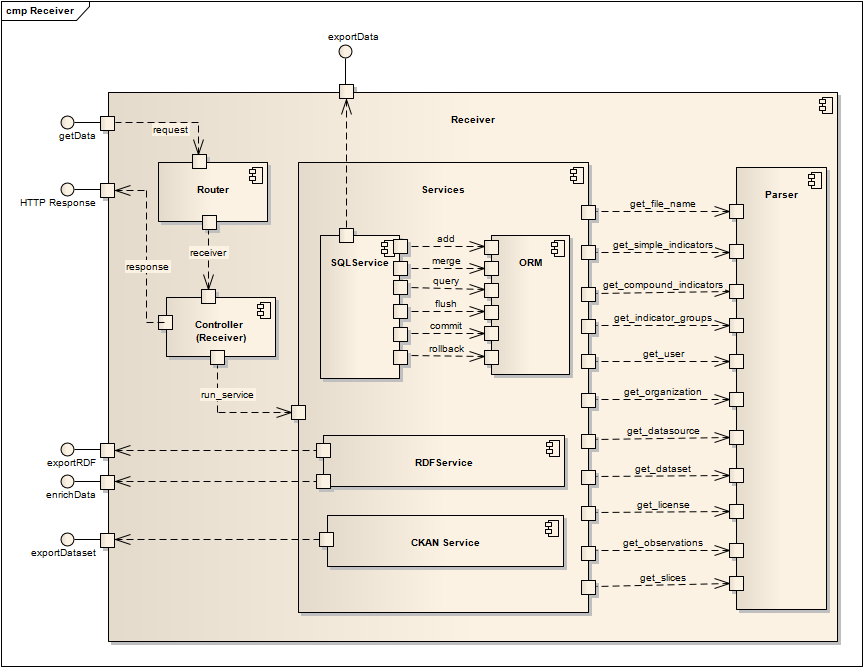
\includegraphics[height=\textwidth]{arquitectura/receiver_view}
		\caption{Diagrama de componentes del punto de entrada de datos}
		\label{fig:diagrama_componentes_receiver}
	\end{figure}
\end{landscape}


\subsubsection{Descripción de los componentes}
Tras haber mostrado el diagrama de los componentes que forman parte del punto de entrada de datos es el momento de explicar el papel que juega cada uno de ellos.

\begin{description}
	\item[Router]  El enrutador se encarga de dirigir las peticiones HTTP que provienen del exterior hacia el controlador.  También es el encargado de responder a las peticiones que no se correspondan con ningún controlador, o que no utilicen un verbo adecuado.
	\item[Controller (Receiver)]  El controlador se encarga de las peticiones de inserción de datos.  Su misión es comprobar si la petición que recibe tiene una forma adecuada y llamar a los distintos servicios para que procesen los datos.
	\item[Parser]  El parser es el encargado de transformar los datos provenientes de las peticiones externas a un modelo de datos que será utilizado por los servicios para realizar los diferentes procesados.  El modelo de datos será visto con más detalle en la sección ``\nameref{diseno_modelo_datos}'' de este mismo capítulo.
	\item[SQLService]  El servicio de SQL se encarga de procesar los datos que llegan al punto de entrada y generar las consultas necesarias para almacenarlos en una base de datos relacional.  Este servicio delega la generación de consultas SQL al ORM.
	\item[ORM]  El Mapeador Objeto-Relacional actúa como una capa de abstracción sobre la base de datos y permite al desarrollador trabajar con objetos sin necesidad de ocuparse de su transformación al modelo relacional.
	\item[RDFService]  El servicio de RDF se encarga de procesar los datos que llegan al punto de entrada y generar los grafos RDF que serán almacenados en el servidor semántico.
	\item[CKANService]  El servicio de CKAN se encarga de procesar los datos que llegan al punto de entrada y generar los metadatos que se almacenan en el catálogo de datos.
\end{description}


\subsubsection{Relacion entre los componentes}
Las peticiones provenientes de los importadores llegan al enrutador.  El enrutador redirige las peticiones que utilicen un verbo adecuado (POST) hacia el controlador, quien comprueba si la petición cuenta con todos los parámetros necesarios.

Si la petición cuenta con los parámetros adecuados, el controlador llama a cada uno de los servicios para que realicen su trabajo.  Los distintos servicios utilizarán a su vez el parser para convertir la información que proviene de la petición a un modelo de datos con el que ellos pueden trabajar.


\subsubsection{Interfaces y puertos}
A continuación se detallarán las interfaces y puertos de los componentes que forman parte del punto de entrada de datos. 

\paragraph{Receiver} \hfill \\
La tabla \ref{interfaces_receiver_receiver} muestra el detalle de las interfaces del \textit{Receiver}.
\begin{longtable}[c]{|p{25mm}|p{20mm}|p{30mm}|p{60mm}|}
 \caption{Vista del punto de entrada de datos - interfaces del \textit{Receiver}.\label{interfaces_receiver_receiver}}\\

 %Cabecera en la primera pagina
 \hline
 	Interfaz & Tipo & Tecnología & Propiedades\\
 \hline
 \hline
 \endfirsthead
 %Cabecera en el resto de páginas
 \hline
 \multicolumn{4}{|c|}{Continuación de la tabla \ref{interfaces_receiver_receiver}}\\
 \hline
 	Interfaz & Tipo & Tecnología & Propiedades\\
 \hline
 \hline
 \endhead
 %Tabla
 \hline
 \endfoot
 
	\textbf{HTTP Request} & Proveída & Servicio web REST & Recibe las peticiones procedentes del exterior \\
	\hline
		
	\textbf{HTTP Response} & Proveída & Servicio web REST & Responde a las peticiones HTTP recibidas \\
	\hline
	
	\textbf{exportRDF} & Requerida & API del servidor semántico & Exporta en formato RDF los datos recibidos de la petición \\
	\hline
	
	\textbf{exportData} & Requerida & Consultas a base de datos & Exporta en formato SQL los datos recibidos de la petición \\
	\hline
	
	\textbf{exportDataset} & Requerida & API del catálogo de datos & Exporta el catálogo de datos recibido de la petición junto con sus metadatos \\
	\hline
	
	\textbf{enrichData} & Requerida & Consultas SPARQL & Enriquece los datos mediante consultas SPARQL a servidores semánticos externos \\
\hline
\hline

 \end{longtable}
 
 
 \paragraph{Router} \hfill \\
 La tabla \ref{interfaces_receiver_router} muestra el detalle de las interfaces del \textit{Router}.
 \begin{longtable}[c]{|p{25mm}|p{20mm}|p{30mm}|p{60mm}|}
  \caption{Vista del punto de entrada de datos - interfaces del \textit{Router}.\label{interfaces_receiver_router}}\\
 
  %Cabecera en la primera pagina
  \hline
  	Interfaz & Tipo & Tecnología & Propiedades\\
  \hline
  \hline
  \endfirsthead
  %Cabecera en el resto de páginas
  \hline
  \multicolumn{4}{|c|}{Continuación de la tabla \ref{interfaces_receiver_router}}\\
  \hline
  	Interfaz & Tipo & Tecnología & Propiedades\\
  \hline
  \hline
  \endhead
  %Tabla
  \hline
  \endfoot
  
 	\textbf{HTTP Request} & Puerto de entrada & Servicio web REST & Recibe las peticiones procedentes del exterior \\
 	\hline
 	
 	\textbf{receiver} & Puerto de salida & Llamada a método & Pasa la petición al controlador correspondiente tras haber comprobado que utiliza el verbo adecuado \\
 \hline
 \hline
 
  \end{longtable}
  
\paragraph{Controller} \hfill \\
La tabla \ref{interfaces_receiver_controller} muestra el detalle de las interfaces del \textit{Controller}.

\begin{longtable}[c]{|p{25mm}|p{20mm}|p{30mm}|p{60mm}|}
 \caption{Vista del punto de entrada de datos - interfaces del textit{Controller}.\label{interfaces_receiver_controller}}\\
   %Cabecera en la primera pagina
 \hline
 	Interfaz & Tipo & Tecnología & Propiedades\\
 \hline
 \hline
 \endfirsthead
 %Cabecera en el resto de páginas
 \hline
 \multicolumn{4}{|c|}{Continuación de la tabla \ref{interfaces_receiver_controller}}\\
 \hline
 	Interfaz & Tipo & Tecnología & Propiedades\\
 \hline
 \hline
 \endhead
 %Tabla
 \hline
 \endfoot
 	
 	\textbf{receiver} & Puerto de entrada & Llamada a método & Recibe la petición procedente el enrutador y comprueba si incluye todos los parámetros necesarios \\
 	\hline
 	
 	\textbf{run service} & Puerto de salida & Llamada a método & Ejecuta la funcionalidad de un servicio \\
 	\hline
 	
 	\textbf{response} & Puerto de salida & Servicio web REST & Envía una respuesta con un código de error HTTP adecuado en función del éxito o no en el procesamiento de la petición. \\
\hline
\hline
 
\end{longtable}


\paragraph{Interfaces comunes a todos los servicios} \hfill \\
La tabla \ref{interfaces_receiver_services} muestra el detalle de las interfaces comunes a todos los servicios.

\begin{longtable}[c]{|p{25mm}|p{20mm}|p{30mm}|p{60mm}|}
 \caption{Vista del punto de entrada de datos - interfaces comunes a todos los servicios.\label{interfaces_receiver_services}}\\
 %Cabecera en la primera pagina
 \hline
 	Interfaz & Tipo & Tecnología & Propiedades\\
 \hline
 \hline
 \endfirsthead
 %Cabecera en el resto de páginas
 \hline
 \multicolumn{4}{|c|}{Continuación de la tabla \ref{interfaces_receiver_services}}\\
 \hline
 	Interfaz & Tipo & Tecnología & Propiedades\\
 \hline
 \hline
 \endhead
 %Tabla
 \hline
 \endfoot
 
 	\textbf{run service} & Puerto de entrada & Llamada a método & Comienza la ejecución del servicio \\
 	\hline
 	
 	\textbf{get file name} & Puerto de salida & Llamada a método & Obtiene el nombre del fichero que contiene los datos en bruto \\
 	\hline
 	
 	\textbf{get simple indicators} & Puerto de salida & Llamada a método & Obtiene una lista de los indicadores simples obtenidos del fichero de datos \\
 	\hline
 	
 	\textbf{get compound indicators} & Puerto de salida & Llamada a método & Obtiene una lista de los indicadores compuestos obtenidos del fichero de datos \\
 	\hline
 	
  	\textbf{get user} & Puerto de salida & Llamada a método & Obtiene los del usuario que realiza la petición de inserción de datos \\
  	\hline
  	
  	\textbf{get organization} & Puerto de salida & Llamada a método & Obtiene la información sobre la organización que proporciona el fichero de datos \\
  	\hline
  	
   	\textbf{get datasource} & Puerto de salida & Llamada a método & Obtiene la información sobre la fuente de datos de la que procede el fichero de datos \\
   	\hline
   	
   	\textbf{get dataset} & Puerto de salida & Llamada a método & Obtiene la información sobre el propio fichero de datos\\
   	\hline
   	
   	\textbf{get license} & Puerto de salida & Llamada a método & Obtiene la información sobre la licencia bajo la que se publica el fichero de datos \\
   	\hline
   	
   	\textbf{get observations} & Puerto de salida & Llamada a método & Obtiene la lista de observaciones procedentes del fichero de datos \\
   	\hline
   	
   	\textbf{get slices} & Puerto de salida & Llamada a método & Obtiene la lista con las \textit{slices}\footnote{Para más información sobre las \textit{slices} véase la sección ``\nameref{concept:rdf_data_cube}'' perteneciente al capítulo \ref{chapter03}} procedentes del fichero de datos. \\
   	\hline
\hline
\hline
 
\end{longtable}


\paragraph{Interfaces del \textit{Parser}} \hfill \\
La tabla \ref{interfaces_receiver_parser} muestra el detalle de las interfaces pertenecientes al \textit{Parser}.

\begin{longtable}[c]{|p{25mm}|p{20mm}|p{30mm}|p{60mm}|}
 \caption{Vista del punto de entrada de datos - interfaces pertenecientes al \textit{Parser}.\label{interfaces_receiver_parser}}\\
 %Cabecera en la primera pagina
 \hline
 	Interfaz & Tipo & Tecnología & Propiedades\\
 \hline
 \hline
 \endfirsthead
 %Cabecera en el resto de páginas
 \hline
 \multicolumn{4}{|c|}{Continuación de la tabla \ref{interfaces_receiver_parser}}\\
 \hline
 	Interfaz & Tipo & Tecnología & Propiedades\\
 \hline
 \hline
 \endhead
 %Tabla
 \hline
 \endfoot
 	
 	\textbf{get file name} & Puerto de entrada & Llamada a método & Devuelve el nombre del fichero que contiene los datos en bruto \\
 	\hline
 	
 	\textbf{get simple indicators} & Puerto de entrada & Llamada a método & Devuelve una lista de los indicadores simples obtenidos del fichero de datos \\
 	\hline
 	
 	\textbf{get compound indicators} & Puerto de entrada & Llamada a método & Devuelve una lista de los indicadores compuestos obtenidos del fichero de datos \\
 	\hline
 	
  	\textbf{get user} & Puerto de salida & Llamada a entrada & Devuelve los del usuario que realiza la petición de inserción de datos \\
  	\hline
  	
  	\textbf{get organization} & Puerto de entrada & Llamada a método & Devuelve la información sobre la organización que proporciona el fichero de datos \\
  	\hline
  	
   	\textbf{get datasource} & Puerto de entrada & Llamada a método & Devuelve la información sobre la fuente de datos de la que procede el fichero de datos \\
   	\hline
   	
   	\textbf{get dataset} & Puerto de entrada & Llamada a método & Devuelve la información sobre el propio fichero de datos\\
   	\hline
   	
   	\textbf{get license} & Puerto de entrada & Llamada a método & Devuelve la información sobre la licencia bajo la que se publica el fichero de datos \\
   	\hline
   	
   	\textbf{get observations} & Puerto de entrada & Llamada a método & Devuelve la lista de observaciones procedentes del fichero de datos \\
   	\hline
   	
   	\textbf{get slices} & Puerto de entrada & Llamada a método & Devuelve la lista con las \textit{slices} procedentes del fichero de datos. \\
   	\hline
\hline
\hline
 
\end{longtable}


\paragraph{SQLService} \hfill \\
La tabla \ref{interfaces_receiver_sqlservice} muestra el detalle de las interfaces del \textit{servicio de SQL} que no han sido incluidas anteriormente en la tabla \ref{interfaces_receiver_services}.  

\begin{longtable}[c]{|p{25mm}|p{20mm}|p{30mm}|p{60mm}|}
	\caption{Vista del punto de entrada de datos - interfaces del \textit{servicio de SQL}.\label{interfaces_receiver_sqlservice}}\\
	%Cabecera en la primera pagina
		\hline
			Interfaz & Tipo & Tecnología & Propiedades\\
		\hline
		\hline
	\endfirsthead
	%Cabecera en el resto de páginas
		\hline
		\multicolumn{4}{|c|}{Continuación de la tabla \ref{interfaces_receiver_sqlservice}}\\
		\hline
			Interfaz & Tipo & Tecnología & Propiedades\\
		\hline
		\hline
	\endhead
	%Tabla
	\hline
	\endfoot
		\textbf{exportData} & Requerida & Consultas a base de datos & Exporta en formato SQL los datos recibidos de la petición \\
		\hline
		\textbf{add} & Puerto de salida & Llamada a método & Almacena los datos de un objeto del modelo en la base de datos \\
		\hline
		\textbf{merge} & Puerto de salida & Llamada a método & Actualiza los datos de un objeto del modelo en la base de datos \\
		\hline
		\textbf{query} & Puerto de salida & Llamada a método & Realiza una consulta a la base de datos y devuelve los resultados\\
		\hline
		\textbf{flush} & Puerto de salida & Llamada a método & Vuelca los cambios realizados en memoria a la base de datos \\
		\hline
		\textbf{commit} & Puerto de salida & Llamada a método & Cierra una transacción con la base de datos \\
		\hline
		\textbf{rollback} & Puerto de salida & Llamada a método & Deshace los cambios de la transacción en curso\\
		\hline
	\hline
	\hline
\end{longtable}


\paragraph{ORM} \hfill \\
La tabla \ref{interfaces_receiver_orm} muestra el detalle de las interfaces del \textit{ORM}.  

\begin{longtable}[c]{|p{25mm}|p{20mm}|p{30mm}|p{60mm}|}
	\caption{Vista del punto de entrada de datos - interfaces del \textit{ORM}.\label{interfaces_receiver_orm}}\\
	%Cabecera en la primera pagina
		\hline
			Interfaz & Tipo & Tecnología & Propiedades\\
		\hline
		\hline
	\endfirsthead
	%Cabecera en el resto de páginas
		\hline
		\multicolumn{4}{|c|}{Continuación de la tabla \ref{interfaces_receiver_orm}}\\
		\hline
			Interfaz & Tipo & Tecnología & Propiedades\\
		\hline
		\hline
	\endhead
	%Tabla
	\hline
	\endfoot
		\textbf{add} & Puerto de entrada & Llamada a método & Almacena los datos de un objeto del modelo en la base de datos \\
		\hline
		\textbf{merge} & Puerto de entrada & Llamada a método & Actualiza los datos de un objeto del modelo en la base de datos \\
		\hline
		\textbf{query} & Puerto de entrada & Llamada a método & Realiza una consulta a la base de datos y devuelve los resultados\\
		\hline
		\textbf{flush} & Puerto de entrada & Llamada a método & Vuelca los cambios realizados en memoria a la base de datos \\
		\hline
		\textbf{commit} & Puerto de entrada & Llamada a método & Cierra una transacción con la base de datos \\
		\hline
		\textbf{rollback} & Puerto de entrada & Llamada a método & Deshace los cambios de la transacción en curso\\
		\hline
	\hline
	\hline
\end{longtable}


\paragraph{RDFService} \hfill \\
La tabla \ref{interfaces_receiver_rdfservice} muestra el detalle de las interfaces del \textit{servicio de RDF} que no han sido incluidas anteriormente en la tabla \ref{interfaces_receiver_services}.  

\begin{longtable}[c]{|p{25mm}|p{20mm}|p{30mm}|p{60mm}|}
	\caption{Vista del punto de entrada de datos - interfaces del \textit{servicio de RDF}.\label{interfaces_receiver_rdfservice}}\\
	%Cabecera en la primera pagina
		\hline
			Interfaz & Tipo & Tecnología & Propiedades\\
		\hline
		\hline
	\endfirsthead
	%Cabecera en el resto de páginas
		\hline
		\multicolumn{4}{|c|}{Continuación de la tabla \ref{interfaces_receiver_rdfservice}}\\
		\hline
			Interfaz & Tipo & Tecnología & Propiedades\\
		\hline
		\hline
	\endhead
	%Tabla
	\hline
	\endfoot
		\textbf{exportRDF} & Requerida & API del servidor semántico & Exporta en formato RDF los datos recibidos de la petición \\
		\hline
		\textbf{enrichData} & Requerida & Consultas SPARQL & Enriquece los datos mediante consultas SPARQL a servidores semánticos externos \\
	\hline
	\hline
\end{longtable}


\paragraph{CKANService} \hfill \\
La tabla \ref{interfaces_receiver_ckanservice} muestra el detalle de las interfaces del \textit{servicio de CKAN} que no han sido incluidas anteriormente en la tabla \ref{interfaces_receiver_services}.  

\begin{longtable}[c]{|p{25mm}|p{20mm}|p{30mm}|p{60mm}|}
	\caption{Vista del punto de entrada de datos - interfaces del \textit{servicio de CKAN}.\label{interfaces_receiver_ckanservice}}\\
	%Cabecera en la primera pagina
		\hline
			Interfaz & Tipo & Tecnología & Propiedades\\
		\hline
		\hline
	\endfirsthead
	%Cabecera en el resto de páginas
		\hline
		\multicolumn{4}{|c|}{Continuación de la tabla \ref{interfaces_receiver_ckanservice}}\\
		\hline
			Interfaz & Tipo & Tecnología & Propiedades\\
		\hline
		\hline
	\endhead
	%Tabla
	\hline
	\endfoot
		\textbf{exportDataset} & Requerida & API del catálogo de datos & Exporta el catálogo de datos recibido de la petición junto con sus metadatos \\
	\hline
	\hline
\end{longtable}


\subsection{Vista de los módulos del gestor de contenidos}
\label{vista_modulos_cms}
A continuación se detallará la estructura completa del gestor de contenidos.  Como se ha explicado en la sección ``\nameref{chapter02:alternativas_seleccionadas}'' perteneciente al capítulo \ref{chapter02}, el gestor de contenidos seleccionado ha sido Drupal.


\subsubsection{Diagrama de componentes}
La figura \ref{fig:diagrama_componentes_cms} muestra el diagrama de los componentes que forman parte del gestor de contenidos.
\begin{landscape}
	\begin{figure}[ht]
		\centering
		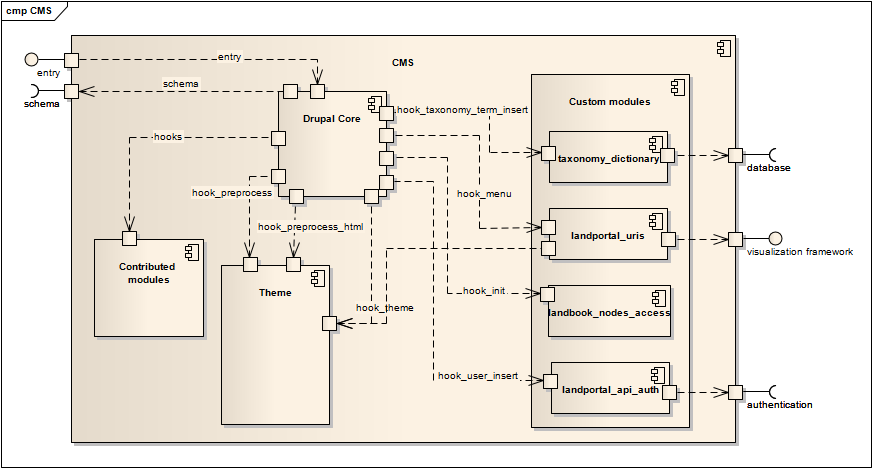
\includegraphics[height=\textwidth]{arquitectura/cms_view}
		\caption{Diagrama de componentes del gestor de contenidos}
		\label{fig:diagrama_componentes_cms}
	\end{figure}
\end{landscape}


\subsubsection{Descripción de los componentes}
Se describirán ahora los distintos componentes que forman parte del gestor de contenidos.
\begin{description}
	\item[Drupal Core]  El núcleo de Drupal implementa la funcionalidad principal del gestor de contenidos.  Es el encargado de procesar y responder a las peticiones, además de coordinar el funcionamiento de los diferentes módulos y temas visuales.
	\item[Contributed modules]  Los módulos contribuidos son módulos realizados por terceros y que han sido públicamente incluidos en el repositorio de módulos de Drupal.  Éstos módulos amplían la funcionalidad existente en el núcleo de Drupal\footnote{Actualmente existen unos 15.000 módulos que forman parte del repositorio.  Dichos módulos pueden verse en \url{https://www.drupal.org/project/project_module}}.
	\item[Custom modules]  Los módulos propios han sido especialmente creados para éste proyecto y realizan alguna funcionalidad que no forma parte del núcleo de Drupal ni de ningún módulo contribuido.  Se han desarrollado cuatro módulos propios:
		\begin{itemize}
			\item \textit{taxonomy\_dictionary}  Permite relacionar los datos existentes en la base de datos con los términos de las taxonomías existentes en Drupal.
			\item \textit{landportal\_uris}  Implementa un sistema similar al MVC para facilitar la creación de vistas.  También incluye el framework que provee de datos a las visualizaciones.  Éste módulo se verá con más detalle posteriormente en la sección ``\nameref{vista_landportal_uris}'' de éste mismo capítulo.
			\item \textit{landbook\_nodes\_access}  Permite redirigir a las vistas adecuadas cuando se visite alguno de los nodos de la sección de datos.
			\item \textit{landportal\_api\_auth}  Genera y almacena las claves de autenticación del el API para los nuevos usuarios que se creen en el sistema.
		\end{itemize}
	\item[Theme]  El tema implementa la interfaz de las diferentes vistas que forman parte del gestor de contenidos.
\end{description}


\subsubsection{Relación entre los componentes}
Las peticiones entrantes son procesadas por el núcleo de Drupal.  En cada petición el núcleo de Drupal invoca los módulos que estén suscritos a los \textit{hooks} adecuados para que realicen su funcionalidad\footnote{El módulo ``\textit{landportal\_uris}'' será detallado posteriormente en la sección ``\nameref{vista_landportal_uris}'' de éste mismo capítulo.  El resto de módulos propios cuentan simplemente con un único fichero que implementa el \textit{hook} correspondiente por lo que, dada su sencillez, sus vistas se omitirán}:
\begin{itemize}
	\item Cuando se crea un nuevo término en la taxonomía se invoca al módulo \textit{taxonomy\_dictionary} para que lo enlace con el término correspondiente en la base de datos.
	\item Cuando se realiza una petición que no va dirigida a mostrar la vista de administración se invoca al módulo \textit{landportal\_uris} para que provea los datos con los que se renderizarán posteriormente las vistas del tema.  Éste procedimiento será posteriormente detallado en la sección INCLUIR SECCION.
	\item Cuando se accede a alguno de los nodos pertenecientes a la zona de datos se invoca al módulo \textit{landbook\_nodes\_access} para que realice la redirección hacia la vista adecuada.
	\item Cuando se crea un nuevo usuario en el portal se invoca al módulo \textit{landportal\_api\_auth} para que cree y almacene sus claves de acceso al API.
\end{itemize}
Por último, el núcleo de Drupal invoca al tema para que renderice las vistas que serán mostradas al usuario que realiza la petición.


\subsubsection{Interfaces y puertos}
A continuación se detallarán las interfaces y puertos de los componentes que forman parte del gestor de contenidos. 

\paragraph{CMS} \hfill \\
La tabla \ref{interfaces_cms_cms} muestra el detalle de las interfaces del \textit{CMS}.

\begin{longtable}[c]{|p{25mm}|p{20mm}|p{30mm}|p{60mm}|}
 \caption{Vista del gestor de contenidos - interfaces del \textit{CMS}.\label{interfaces_cms_cms}}\\

 %Cabecera en la primera pagina
 \hline
 	Interfaz & Tipo & Tecnología & Propiedades\\
 \hline
 \hline
 \endfirsthead
 %Cabecera en el resto de páginas
 \hline
 \multicolumn{4}{|c|}{Continuación de la tabla \ref{interfaces_receiver_receiver}}\\
 \hline
 	Interfaz & Tipo & Tecnología & Propiedades\\
 \hline
 \hline
 \endhead
 %Tabla
 \hline
 \endfoot
 
	\textbf{entry} & Proveída & Petición HTTP & Recibe las peticiones procedentes del exterior \\
	\hline
		
	\textbf{schema} & Requerida & API del motor de búsqueda & Envía los datos del gestor de contenidos al motor de búsqueda para su indexación\footnote{ Como se ha explicado en la sección ``\nameref{chapter02:alternativas_seleccionadas}'' perteneciente al capítulo \ref{chapter02}, el motor de búsqueda seleccionado ha sido \textit{Apache Solr}} \\
	\hline
	
	\textbf{database} & Requerida & Conexión a base de datos & Accede a la base de datos donde se almacena la información perteneciente al subsistema de datos \\
	\hline
	
	\textbf{visualization framework} & Proveída & API Web & Provee datos con los que posteriormente crear las visualizaciones\footnote{Los elementos de éste framework podrán ser vistos con mayor detalle posteriormente en la sección ``\nameref{vista_landportal_uris}'' perteneciente a éste mismo capítulo} \\
	\hline
	
	\textbf{authentication} & Proveída & API REST & Genera claves de autenticación en el API para los usuarios del portal \\
\hline
\hline

 \end{longtable}


\paragraph{Drupal Core} \hfill \\
La tabla \ref{interfaces_cms_drupalcore} muestra el detalle de las interfaces del \textit{núcleo de Drupal}.  

\begin{longtable}[c]{|p{25mm}|p{20mm}|p{30mm}|p{60mm}|}
	\caption{Vista del gestor de contenidos - interfaces del \textit{núcleo de Drupal}.\label{interfaces_cms_drupalcore}}\\
	%Cabecera en la primera pagina
		\hline
			Interfaz & Tipo & Tecnología & Propiedades\\
		\hline
		\hline
	\endfirsthead
	%Cabecera en el resto de páginas
		\hline
		\multicolumn{4}{|c|}{Continuación de la tabla \ref{interfaces_cms_drupalcore}}\\
		\hline
			Interfaz & Tipo & Tecnología & Propiedades\\
		\hline
		\hline
	\endhead
	%Tabla
	\hline
	\endfoot
		\textbf{entry} & Puerto de entrada & Petición HTTP & Recibe las peticiones procedentes del exterior \\
		\hline
		
		\textbf{schema} & Puerto de salida & API del motor de búsqueda & Envía los datos del gestor de contenidos al motor de búsqueda para su indexación \\
		\hline
		
		\textbf{hooks} & Puerto de salida & Llamada a método & Invoca a los módulos que estén suscritos al \textit{hook} correspondiente \\
		\hline
		
		\textbf{hook preprocess} & Puerto de salida & Llamada a método & Indica al tema que preprocese las variables que sean necesarias para las vistas \\
		\hline
		
		\textbf{hook preprocess html} & Puerto de salida & Llamada a método & Indica al tema que preprocese las variables que sean necesarias para la plantilla HTML \\
		\hline
		
		\textbf{hook theme} & Puerto de salida & Llamada a método & Indica al tema que renderice una determinada plantilla para una vista \\
		\hline
		
		\textbf{hook taxonomy term insert} & Puerto de salida & Llamada a método & Indica a un módulo que se ha creado un nuevo término en la taxonomía para que éste realice su funcionalidad \\
		\hline
		
		\textbf{hook menu} & Puerto de salida & Llamada a método & Permite a un módulo registrar rutas para definir cómo son atendidas las peticiones HTTP \\
		\hline
		
		\textbf{hook init} & Puerto de salida & Llamada a método & Indica a un módulo que acaba de tener lugar una petición por parte de un usuario \\
		\hline
		
		\textbf{hook user insert} & Puerto de salida & Llamada a método & Indica a un módulo que acaba de producirse el registro de un nuevo usuario \\
	\hline
	\hline
\end{longtable}


\paragraph{Contributed modules} \hfill \\
La tabla \ref{interfaces_cms_modules} muestra el detalle de las interfaces de los \textit{módulos contribuidos}.  

\begin{longtable}[c]{|p{25mm}|p{20mm}|p{30mm}|p{60mm}|}
	\caption{Vista del gestor de contenidos - interfaces de los \textit{módulos contribuidos}.\label{interfaces_cms_modules}}\\
	%Cabecera en la primera pagina
		\hline
			Interfaz & Tipo & Tecnología & Propiedades\\
		\hline
		\hline
	\endfirsthead
	%Cabecera en el resto de páginas
		\hline
		\multicolumn{4}{|c|}{Continuación de la tabla \ref{interfaces_cms_modules}}\\
		\hline
			Interfaz & Tipo & Tecnología & Propiedades\\
		\hline
		\hline
	\endhead
	%Tabla
	\hline
	\endfoot
		\textbf{hooks} & Puerto de entrada & Llamada a método & Invocados por el núcleo de Drupal cuando tienen lugar ciertos eventos en el sistema \\
	\hline
	\hline
\end{longtable}


\paragraph{Theme} \hfill \\
La tabla \ref{interfaces_cms_theme} muestra el detalle de las interfaces del \textit{tema}.  

\begin{longtable}[c]{|p{25mm}|p{20mm}|p{30mm}|p{60mm}|}
	\caption{Vista del gestor de contenidos - interfaces del \textit{tema}.\label{interfaces_cms_theme}}\\
	%Cabecera en la primera pagina
		\hline
			Interfaz & Tipo & Tecnología & Propiedades\\
		\hline
		\hline
	\endfirsthead
	%Cabecera en el resto de páginas
		\hline
		\multicolumn{4}{|c|}{Continuación de la tabla \ref{interfaces_cms_theme}}\\
		\hline
			Interfaz & Tipo & Tecnología & Propiedades\\
		\hline
		\hline
	\endhead
	%Tabla
	\hline
	\endfoot
		\textbf{hook preprocess} & Puerto de entrada & Llamada a método & Preprocesa las variables que sean necesarias para la posterior renderización de las vistas \\
		\hline
			
		\textbf{hook preprocess html} & Puerto de entrada & Llamada a método & Preprocesa las variables necesarias para renderizar la plantilla HTML \\
		\hline
			
		\textbf{hook theme} & Puerto de entrada & Llamada a método & Renderiza la plantilla de una determinada vista \\
	\hline
	\hline
\end{longtable}


\paragraph{Taxonomy dictionary} \hfill \\
La tabla \ref{interfaces_cms_taxonomy_dictionary} muestra el detalle de las interfaces del módulo ``\textit{Taxonomy dictionary}''.  

\begin{longtable}[c]{|p{25mm}|p{20mm}|p{30mm}|p{60mm}|}
	\caption{Vista del gestor de contenidos - interfaces del módulo \textit{Taxonomy dictionary}. \label{interfaces_cms_taxonomy_dictionary}}\\
	%Cabecera en la primera pagina
		\hline
			Interfaz & Tipo & Tecnología & Propiedades\\
		\hline
		\hline
	\endfirsthead
	%Cabecera en el resto de páginas
		\hline
		\multicolumn{4}{|c|}{Continuación de la tabla \ref{interfaces_cms_taxonomy_dictionary}}\\
		\hline
			Interfaz & Tipo & Tecnología & Propiedades\\
		\hline
		\hline
	\endhead
	%Tabla
	\hline
	\endfoot
		\textbf{hook taxonomy term insert} & Puerto de entrada & Llamada a método & Recibe la información de un nuevo término que se ha creado en la taxonomía \\
		\hline
		\textbf{database} & Puerto de salida & Conexión a base de datos & Almacena la información del término insertado en la taxonomía en la entrada correspondiente de la base de datos \\
	\hline
	\hline
\end{longtable}


\paragraph{LandPortal URIs} \hfill \\
La tabla \ref{interfaces_cms_landportal_uris} muestra el detalle de las interfaces del módulo ``\textit{LandPortal URIs}''.  

\begin{longtable}[c]{|p{25mm}|p{20mm}|p{30mm}|p{60mm}|}
	\caption{Vista del gestor de contenidos - interfaces del módulo \textit{LandPortal URIs}. \label{interfaces_cms_landportal_uris}}\\
	%Cabecera en la primera pagina
		\hline
			Interfaz & Tipo & Tecnología & Propiedades\\
		\hline
		\hline
	\endfirsthead
	%Cabecera en el resto de páginas
		\hline
		\multicolumn{4}{|c|}{Continuación de la tabla \ref{interfaces_cms_landportal_uris}}\\
		\hline
			Interfaz & Tipo & Tecnología & Propiedades\\
		\hline
		\hline
	\endhead
	%Tabla
	\hline
	\endfoot
		\textbf{hook menu} & Puerto de entrada & Llamada a método & El gestor de contenidos está definiendo las rutas que tendrán las vistas del portal \\
		\hline
		\textbf{hook theme} & Puerto de salida & Llamada a método & Indica al tema que renderice una determinada plantilla para una vista \\
		\hline
		\textbf{visualization framework} & Puerto de salida & API Web & Provee datos con los que posteriormente crear las visualizaciones \\
		\hline
		\textbf{database} & Puerto de salida & Conexión a base de datos & Obtiene información de la base de datos \\
	\hline
	\hline
\end{longtable}


\paragraph{LandbBook nodes access} \hfill \\
La tabla \ref{interfaces_cms_landbook_nodes_access} muestra el detalle de las interfaces del módulo ``\textit{LandbBook nodes access}''.  

\begin{longtable}[c]{|p{25mm}|p{20mm}|p{30mm}|p{60mm}|}
	\caption{Vista del gestor de contenidos - interfaces del módulo \textit{LandbBook nodes access}. \label{interfaces_cms_landbook_nodes_access}}\\
	%Cabecera en la primera pagina
		\hline
			Interfaz & Tipo & Tecnología & Propiedades\\
		\hline
		\hline
	\endfirsthead
	%Cabecera en el resto de páginas
		\hline
		\multicolumn{4}{|c|}{Continuación de la tabla \ref{interfaces_cms_landbook_nodes_access}}\\
		\hline
			Interfaz & Tipo & Tecnología & Propiedades\\
		\hline
		\hline
	\endhead
	%Tabla
	\hline
	\endfoot
		\textbf{hook init} & Puerto de entrada & Llamada a método & Invocada por el núcleo del gestor de contenidos cuando acaba de tener lugar una petición por parte de un usuario \\
	\hline
	\hline
\end{longtable}


\paragraph{Landportal API auth} \hfill \\
La tabla \ref{interfaces_cms_landportal_api_auth} muestra el detalle de las interfaces del módulo ``\textit{LandPortal API auth}''.  

\begin{longtable}[c]{|p{25mm}|p{20mm}|p{30mm}|p{60mm}|}
	\caption{Vista del gestor de contenidos - interfaces del módulo \textit{LandPortal API auth}. \label{interfaces_cms_landportal_api_auth}}\\
	%Cabecera en la primera pagina
		\hline
			Interfaz & Tipo & Tecnología & Propiedades\\
		\hline
		\hline
	\endfirsthead
	%Cabecera en el resto de páginas
		\hline
		\multicolumn{4}{|c|}{Continuación de la tabla \ref{interfaces_cms_landportal_api_auth}}\\
		\hline
			Interfaz & Tipo & Tecnología & Propiedades\\
		\hline
		\hline
	\endhead
	%Tabla
	\hline
	\endfoot
		\textbf{hook user insert} & Puerto de entrada & Llamada a método & Invocado por el núcleo del gestor de contenidos cuando se realiza el registro de un nuevo usuario \\
		\hline
		\textbf{authentication} & Puerto de salida & API REST & Genera claves de autenticación en el API para el usuario recién registrado en el portal \\
	\hline
	\hline
\end{longtable}


\subsection{Vista del módulo \textit{landportal uris}}
\label{vista_landportal_uris}